\section{Triple cut, triangle and bubble coefficients in $D=4$}\label{sect-triple_cut}
We are now left with triangle and bubble coefficients to determine. 
A method using triple cut to determine the triangle and bubble coefficients in one-loop in four-dimension was proposed by Forde~\cite{Forde:2007mi}.
This method consists in choosing an appropriate parametrization for the loop momentum after applying cuts such that the triangle and bubble contributions can be distinguished from the box contributions.
In this method, we consider four-dimensional loop momentum.
\begin{figure}[h]
  \centering
  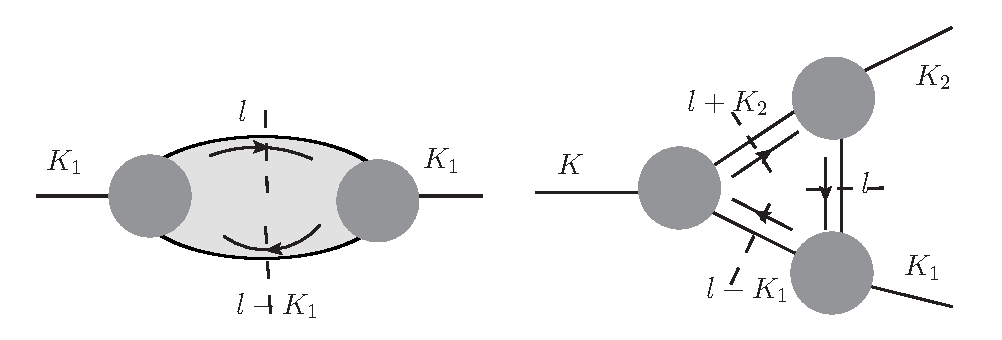
\includegraphics[width=0.8\linewidth]{triple_cut.eps}
  \caption{The two particle cut and triple cut used in this section}
  \label{fig-triple_cut}
\end{figure}
%
\subsection*{Triangle coefficient} 
Upon applying a triple cut, the three delta functions leave only one degree of freedom in four dimensions. 
Let us denote it by $t$.
The most general expression for a cut amplitude takes the form 
\begin{equation}\label{tricut}
(2\pi)^3\int\dd l^4 \prod_{i=0}^2 \delta(l_i^2) A_1A_2A_3 = 
(2\pi)^3\int\dd l^4 \prod_{i=0}^2 \delta(l_i^2)\Big(\mathrm{Inf}_t(A_1A_2A_3)(t) + \sum_{\textrm{$t_j$ poles}}\frac{\res_{t = t_j}A_1 A_2 A_3}{t-t_j}\Big)
\end{equation}
where the $A$'s are tree amplitudes and the first term on the right-hand side is a polynomial in $t$ defined by
\begin{equation}
\lim_{t\rightarrow\infty}\big([\mathrm{Inf}_tA_1A_2A_3](t) - A_1A_2A_3(t)\big) = 0
\end{equation}
In most of cases, propagators of the type $\frac{1}{(l-P)^2}$ contain two poles that can be expressed in terms of $t$. 
The second part of~\cref{tricut} can hence be considered as contributions of cut boxes. 
As a result, the information on the bubble and triangle contributions is only contained in the first term on the \rhs of~\cref{tricut}.
According to Forde, we can choose a parametrization such that only the constant term in the polynomial $\mathrm{Inf}_t(A_1A_2A_3)(t)$ contributes to the integral. 
%
\\\\
Consider a triple cut leading to the constraints\footnote{Here we take $-K_2$ instead of $K_2$ in the triangle diagram of figure~\ref{fig-triple_cut}, which is the choice used in Forde's original paper.}
\begin{equation}
l^2 = (l-K_1)^2 = (l - K_2)^2 = 0
\end{equation}
One can construct two null vectors $K_1^\flat$ and $K_2^\flat$ from the external momenta $K_1$ and $K_2$ 
\begin{equation}\label{k_flat}
K_1^\flat = K_1 - \frac{S_1}{\gamma}K_2^\flat \quad\quad
K_2^\flat = K_2 - \frac{S_2}{\gamma}K_1^\flat
\end{equation}
%
where $S_i = K_i^2$ and $\gamma = \langle K_1^\flat|\slashed{K}_2^\flat|K_1^\flat] =\langle K_2^\flat|\slashed{K}_1^\flat|K_2^\flat]$.
There are two possibilities for $\gamma$
\begin{equation}\label{sol_for_gamma}
\gamma_{\pm} = (K_1\cdot K_2) \pm\sqrt{\Delta}\quad
\mathrm{where}\quad
\Delta = (K_1\cdot K_2)^2 - K_1^2K_2^2
\end{equation}
In terms of the spinor components, the constraints require
\begin{equation}\label{l_param}
\langle l | = t\langle K_1^\flat| + \alpha_{01}\langle K_2^\flat| 
\quad,\quad
[ l | = \frac{\alpha_{02}}{t}[ K_1^\flat| + [ K_2^\flat|
\end{equation}
where
\begin{equation}
\alpha_{01} = \frac{S_1(\gamma S_2)}{\gamma^2 - S_1S_2}\quad,\quad
\alpha_{02} = \frac{S_2(\gamma S_1)}{\gamma^2 - S_1S_2}
\end{equation}
%
and, as four-vector,
\begin{equation}
l^\mu = \alpha_{02} K_1^{\flat,\mu} + \alpha_{01}K_2^{\flat,\mu} + \frac{t}{2}\langle K_1^\flat | \gamma^\mu |K_2^\flat] + \frac{\alpha_{01}\alpha_{02}}{2t}\langle K_2^\flat|\gamma^\mu |K_1^\flat]
\end{equation}
%
Now, we can use an argument similar to the one in~\cite{Ossola:2006us} on the spurious term to find the vanishing integrals.
%\color{red}Appendix ?\color{black}
%
%%%%%%%%%%%%% not used
\iffalse
To illustrate this argument, we consider the case of a rank-1 3-point-like integral. 
By simple arguments on the rank and the dependence on external momenta, 
\begin{equation}
\int\dd^D q \frac{q^\mu}{D_0(q)D_1(q+p_1)D_2(q+p_2)} = c_1p_1^\mu + c_2p_2^\mu
\end{equation}
If we contract the above relation with a vector $v^\mu$ orthogonal to $p_1$ and $p_2$, we obtain a vanishing integral.
$q\cdot v$ is hence a spurious term.
The same technique can be applied to show that $(q\cdot v)^n$ is spurious for any $n>0$. 
\fi
%%%%%%%%%%%%%%%%%%%5 end of not used
%
We can use 
\begin{equation}
\langle K_1^{\flat,\pm} | K_{1,2}|K_2^{\flat,\pm}\rangle = 0 
\quad\mathrm{and}\quad
\langle K_1^{\flat,\pm}|\gamma^\mu|K_{2}^{\flat,\pm}\rangle\langle K_1^{\flat,\pm}|\gamma_\mu|K_{2}^{\flat,\pm}\rangle = 0
\end{equation}
to show that all only the constant term in the polynomial $\mathrm{Inf}_t(A_1A_2A_3)(t)$ contributes to~\cref{tricut}. 
The other two loop-momenta, $l_1 = l-K_1$ and $l_2 = l-K_2$, are parametrized in a similar way in~\cref{l_param} by replacing $\alpha_{01}$ and $\alpha_{02}$ by $\alpha_{i1}$ and $\alpha_{i2}$ given in~\cite{Forde:2007mi}.
%
%
\subsection*{Double cuts and scalar bubble coefficients}
Triple cuts can also be used to determine bubble coefficients. 
Let us first consider a double cut (cf. figure~\ref{fig-triple_cut}).
Contrary to the previous case, we will have two free parameters $y$ and $t$.
\begin{equation}\label{2-part_cut}
\begin{split}
(2\pi)^2\int \dd^4 l \prod_{i=0}^1 \delta(l_i^2) A_1 A_2 = & 
(2\pi)^2\int \dd t\dd y J_{t,y}\Big(\big[\mathrm{Inf}_t [\mathrm{Inf}_y(A_1A_2)](y)\big](t) 
\\&
+
\mathrm{Inf}_t\big(\sum_{\textrm{poles}}\frac{\mathrm{Res}_{y = y_i}A_1A_2}{y-y_j})
+
\mathrm{Inf}_t\big(\sum_{\textrm{poles}}\frac{\mathrm{Res}_{t = t_l}\mathrm{Inf}_y A_1A_2}{t-t_l})
\\ &
+
\mathrm{Inf}_t\big(\sum_{\textrm{poles}}\frac{\mathrm{Inf}_t\big(\sum_{\textrm{poles}}\frac{\mathrm{Res}_{y = y_i}A_1A_2}{y-y_j}\big)}{t-t_l}\big)
\Big)
\end{split}
\end{equation}
We parametrize the loop momentum $l$ by
\begin{equation}
l^\mu = yK_1^{\flat,\mu} + \frac{S_1}{\gamma}(1-y)\chi^\mu + \frac{t}{2}\langle K_1^\flat|\gamma^\mu|\chi] + \frac{S_1}{2\gamma}\frac{y}{t}(1-y)\langle \chi|\gamma^\mu|K_1^\flat]
\end{equation}
where
\begin{equation}
K_1^\flat = K_1 - \frac{S_1}{\gamma}\chi^\mu ,\quad
\gamma = \langle \chi | \slashed{K}_1^\flat|\chi]
\end{equation}
and $\chi$ is an arbitrary null vector (non-collinear to $K_1$).
\\
As in the triangle case, we can use 
\begin{equation}
\langle K_1^\flat| \slashed{K}_1|\chi] = \langle K_1^\flat|\slashed{K}_1 | \gamma^\mu|\chi]\langle K_1^\flat|\gamma_\mu|\chi]= 0
\end{equation}
to show that
\begin{equation}
\int\dd t\dd y J_{t,y}t^n = \int \dd t \dd y \big(\frac{y}{t}\big)^n(1-y)^n = 0
\quad\Rightarrow\quad
\int \dd t \dd y J_{t,y}t^n = 0
\quad\textrm{for}\quad n\neq 0
\end{equation} 
From the Passarino-Veltman reduction, we are able to conclude that all integrands of the type $t^0y^m$ are non-vanishing, which makes difference \wrt the triple cut case. 
Naively, one might think that the bubble coefficients come from the first term of~\cref{2-part_cut}.
However, the loop momentum parametrization that has been used leads to more non-vanishing terms than in the triple cut case. 
Furthermore, the second and the third terms in~\cref{2-part_cut} can be reduced to scalar bubble integrals plus triangle integrals. 
In order to relate the contribution to the bubble coefficient of the residue piece, we apply an additional constraint: $(l+K_2)^2=0$ to the double cut (where $K_2$ is another external leg).
This will then fix the free parameter $y$.
The integral will then take the form
\begin{equation}
(2\pi)^3\int \dd t \dd y J_t'\big(\delta(y-y_+) + \delta(y-y_-)\big) \mathcal{M}(y,t) = -2(2\pi)^2 i \int \dd t \dd y J_{t,y}\mathrm{Res}_{y = y_{\pm}}\frac{\mathcal{M}(y,t)}{(l+K_2)^2}
\end{equation}
where $\mathcal{M}(y,t)$ is a general cut integral and $J_t'$ a function of $t$.
Therefore, the residue contributions are, up to a factor of $-\frac{1}{2}$, given by the triple cut.
As discussed in the previous subsection, the $t^0$ contribution in the triple cut gives the triangle coefficients ant the other terms in power of $t$ give the scalar bubble coefficients.
\\\\
We will just list here the final result without giving computational details which involve calculations of non-vanishing integrals and reduction techniques.
The bubble coefficient is given by
\begin{equation}
b = -i[\Inf_t[\Inf_y A_1 A_2](y)](t)\big|_{t\rightarrow 0 , y^m\rightarrow \frac{1}{m+1}}
-\frac{1}{2}\sum_{C_{\mathrm{tri}}}[\Inf_t A_1A_2A_3](t)\big|_{t^j\rightarrow T(j)}
\end{equation}
where the subscripts indicate the substitutions to be done and $T(j)$ is given in eq.(5.26) of~\cite{Forde:2007mi}. 
The second term above is summed over all possible triangle configurations.
\\\\
%%%%%% not used
\iffalse
As an example, let us cite briefly how the two-mass linear triangle
\begin{equation}
(2\pi)^2\int\dd^4 l \prod_{i=0}^1\delta(l_i^2)\frac{\langle K_2|\slashed{l}|K_1]}{(l+K_2)^2}
\end{equation}
is treated in~\cite{Forde:2007mi}:
\begin{enumerate}
\item Do a two-particle cut. We will then get two terms in the integrand: one in $y^0$ and a residual term. The term in $y^0$ gives us a contribution to the bubble coefficients; while the residual term means that a triple cut is needed to get the contributions to the bubble and triangle contributions.
%
\item Apply a triple cut. There will be a term in $t$ if we choose the parametrization introduced previously, which encodes information on the bubble coefficients.
%
\item This term then requires the knowledge of $\int \dd t J_t' t$, which can be re-expressed in terms of our parametrization. Then, apply the Passarino-Veltman reduction to get the relationsship between $\int \dd tJ_t' t$ and the cut bubble $B_0^{\mathrm{cut}(K_1^2)}$
\end{enumerate}
\fi
% end of not used
%
%
%
\subsection*{Example: triangle coefficient extraction for six-photon amplitude in QED}
Let us show explicitly how to extract the coefficient for scalar triangle using the example of the six-photon amplitude $A_6[1^-2^+3^-4^+5^-6^+]$ in QED.
This example is given in~\cite{Forde:2007mi}.
\begin{figure}
  \centering
  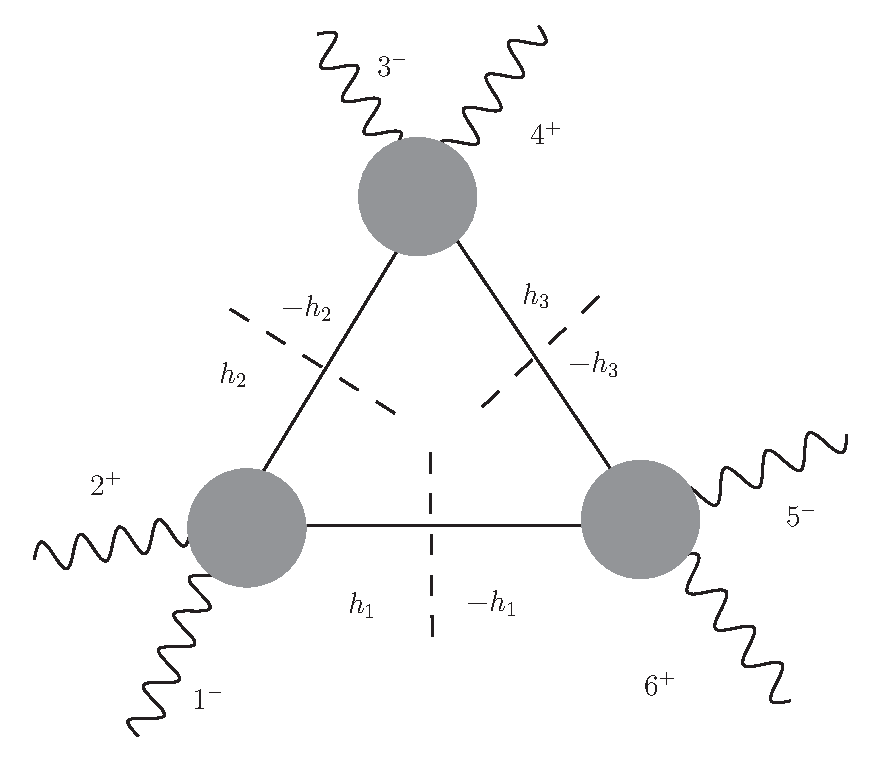
\includegraphics[width=0.5\linewidth]{6photons.eps}
  \caption{Triple cut for the six-photon example}
  \label{fig-6photons}
\end{figure}
First, we have to compute the tree-level four-point amplitude $A_4[1^{h_1}2^{h_2}3^{h_3}4^{h_4}]$. 
Contrary to non-abelian theories, the four-photon amplitude vanishes at tree-level in QED.
Thus, the relevant four-point amplitudes are following ones which contain two photons and two fermions
\begin{equation}
A_4^{\mathrm{tree}}(\bar{f}_1^- f_2^+ \gamma_1^-\gamma_2^+)
\quad,\quad
A_4^{\mathrm{tree}}(\bar{f}_1^+ f_2^- \gamma_1^-\gamma_2^+)
\end{equation}
Recall that the polarization vectors contracted with the $\gamma$-matrices are represented by\footnote{This can be shown using the expression given previously and the Fierz identity.}
\begin{equation}
\begin{split}
& \slashed{\epsilon}_+(p,k) = -\frac{\sqrt{2}}{\langle kp\rangle}\big(|p]\langle k| + |k\rangle[p|\big)
\\
& \slashed{\epsilon}_-(p,k) = \frac{\sqrt{2}}{[kp]}\big(|p\rangle [k| + |k]\langle p|\big)
\end{split}
\end{equation}
We denote the out-going fermion momenta by $q_i$ and the out-going photon momenta by $p_i$. 
A direct Feynman diagram computation gives\footnote{Recall that we take all the particles out-going in our convention.}
\begin{figure}[h]
  \centering
  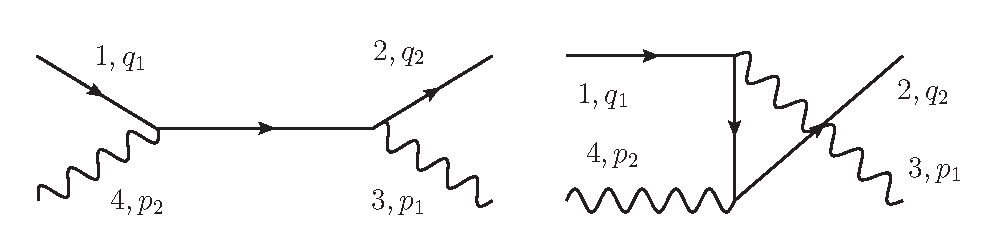
\includegraphics[width=0.8\linewidth]{qed.eps}
  \caption{$s$-channel (left) and $u$-channel (right)}
  \label{fig-qed}
\end{figure}
%
\begin{equation}
\begin{split}
A_{4}^{\mathrm{tree}}(\bar{f}_1^- f_2^+ \gamma_1^-\gamma_2^+) 
= &
\frac{ie^2}{(-p_1 - q_1)^2}\langle q_1, p_1\rangle \frac{\sqrt{2}}{[k, p_1]}
[k|\big(|p_2] \langle p_2| + |q_2]\langle q_2|\big)
\frac{\sqrt{2}}{\langle k p_2\rangle}
\big(|p_2]\langle k| + |k\rangle[p_2|\big) |q_2]
\\
&
+\frac{ie^2}{(-q_1-p_2)^2}\langle q_1, k'\rangle
\frac{\sqrt{2}}{\langle k', p_2\rangle}[p_2|
\big( -|p_2]\langle p_2| - |q_1]\langle q_1|\big)
\frac{\sqrt{2}}{[k', p_1]}|k'\rangle [p_1, q_2]
\end{split}
\end{equation}
The first term corresponds to the $u$-channel (cf. figure~\ref{fig-qed}) and the second to the $s$-channel.
By choosing the reference momentum $k'$ to be $q_1$, the second term above vanishes. 
We can choose $k = q_2$ and get 
\begin{equation}\label{4pt_qed1}
\begin{split}
A_{4}^{\mathrm{tree}}(\bar{f}_1^- f_2^+ \gamma_1^-\gamma_2^+) 
= &
\frac{2ie^2\langle q_1 p_1 \rangle[p_2 q_2]^2}{[q_2 p_1](p_1+q_1)^2}
\\ 
= &
\frac{2ie^2[42]^2}{[23][31]}
\end{split}
\end{equation}
where in the last equation, the particles are indexed in the order in which they appear in the argument of the amplitude.
In the same manner, there is an $u$-channel and an $s$-channel contribution for the other relevant four-point amplitude. 
The $u$-channel can be made vanishing by choosing properly the reference momentum. 
If we choose the reference momentum for the $s$-channel to be $q_2$, we find 
\begin{equation}\label{4pt_qed2}
A_4^{\mathrm{tree}}(\bar{f}_1^+ f_2^- \gamma_1^- \gamma_2^+) = 
\frac{2ie^2\langle 32\rangle^2}{\langle 41 \rangle\langle 24\rangle}
\end{equation}
Applying a triple cut on the channel $12:34:56$ (cf. figure~\ref{fig-6photons}), we get the two contributing cut amplitudes
\begin{equation}\label{triple_cut_1}
A_{4}^{\mathrm{tree}}(f_1^- 1^-2^+\bar{f}_3^+)
A_4^{\mathrm{tree}}(\bar{f}_1^+f_2^-5^-6^+)
A_4^{\mathrm{tree}}(\bar{f}_2^+ f_3^-3^-4^+)
=
-8ie^6\frac{\langle l_1 1\rangle^2 \langle 5l_2 \rangle^2\langle 3l_3\rangle^2}{\langle2 l_3\rangle\langle l_1 2\rangle\langle 6 l_1 \rangle\langle l_2 6\rangle\langle 4 l_2\rangle\langle l_3 4\rangle}
\end{equation}
\begin{equation}\label{triple_cut_2}
A_{4}^{\mathrm{tree}}(f_1^+ 1^-2^+\bar{f}_3^-)
A_4^{\mathrm{tree}}(\bar{f}_1^-f_2^+5^-6^+)
A_4^{\mathrm{tree}}(\bar{f}_2^- f_3^+3^-4^+)
=
-8ie^6\frac{[2l_1]^2[6l_2]^2[4l_3]^2}{[l_1 1 ][1l_3][l_2 5][5l_1][l_2 3][3l_3]}
\end{equation}
where $l_i$ stands for momentum of the outgoing fermion $f_i$.
%
%%%%%%%%%%%%%%%%%%%%%%%%%%%%%%%%%%%%%%%%
\iffalse
Under the triple cut parametrization,~\cref{triple_cut_1} and~\cref{triple_cut_2} lead to the same contribution. 
In fact, the ratio of~\cref{4pt_qed1} to~\cref{4pt_qed2} gives
\begin{equation}
\frac{[42]^2}{[23][31]}\frac{\langle 41\rangle\langle 24\rangle}{\langle 32 \rangle^2} = \frac{\langle 31\rangle[42]}{\langle 32 \rangle[41]} 
\end{equation} 
Hence the ratio of~\cref{triple_cut_1} to~\cref{triple_cut_2} is
\begin{equation}
\frac{[4l_2]\langle 3l_3\rangle}{[4l_3]\langle 3l_2\rangle}
\frac{[6l_1]\langle 5l_2\rangle}{[6l_2]\langle 5l_1\rangle}
\frac{[2l_3]\langle 1l_1\rangle}{[2l_1]\langle 1l_3\rangle}
\end{equation}
\fi
%
%%%%%%%%%%%%%%%%%%%%%%%%%%%%%%%%%%%%%
Because the contribution to triangle coefficient is given by taking the $\Inf$ of~\cref{triple_cut_1} and~\cref{triple_cut_2}, we are interested in the $\Inf$ part of the above under the parametrization~\cref{l_param}, which gives, after some spinor-helicity algebras,
\begin{equation}
\Inf\Big(\frac{([4K_2^\flat] + \frac{\alpha_{12}}{t}[4K_1^\flat])(t\langle 3K_1^\flat \rangle + \alpha_{21}\langle 3K_2^\flat\rangle)}{([4K_2^\flat] + \frac{\alpha_{22}}{t}[4K_1^\flat])(t\langle 3K_1^\flat \rangle + \alpha_{11}\langle 3K_2^\flat\rangle)}(\ldots)\Big)
= 1
\end{equation} 
%
Thus, the total contribution is twice of~\ref{triple_cut_1}, or in a more explicit form using~\cref{l_param}\footnote{
Note that here we apply an offset of one to the indices \wrt the previous notation.
}
\begin{equation}
\begin{split}
-16ie^6 & \frac{(t\langle K_1^\flat 1 \rangle + \alpha_{01}\langle K_2^\flat 1\rangle)^2
(t\langle K_1^\flat 5 \rangle + \alpha_{11}\langle K_2^\flat 5\rangle)^2
(t\langle K_1^\flat 3 \rangle + \alpha_{21}\langle K_2^\flat 3\rangle)^2
}{
(t\langle 2K_1^\flat  \rangle + \alpha_{21}\langle 2 K_2^\flat \rangle)
(t\langle K_1^\flat 2 \rangle + \alpha_{01}\langle K_2^\flat 2\rangle)
(\langle  6K_1^\flat  \rangle + \alpha_{01}\langle  6K_2^\flat \rangle)^2
(t\langle K_1^\flat 6 \rangle + \alpha_{11}\langle K_2^\flat 6\rangle)}
\\
&\times
\frac{1}{
(t\langle 4K_1^\flat  \rangle + \alpha_{11}\langle 4 K_2^\flat \rangle)
(t\langle K_1^\flat 4 \rangle + \alpha_{21}\langle K_2^\flat 4 \rangle)
}
\end{split}
\end{equation}
As a last step, we obtain the triangle coefficient by taking the $\Inf$ of the above and average over all possible solution for the $\gamma_\pm$~\cref{sol_for_gamma}
\begin{equation}
8ie^6\sum_{\gamma_\pm}\frac{\langle K_1^\flat 1 \rangle^2\langle K_1^\flat 5\rangle^5 \langle K_1^\flat 3 \rangle^2}{\langle K_1^\flat 2 \rangle^2\langle K_1^\flat 6\rangle^2 \langle K_1^\flat 4 \rangle^2}
\end{equation}
Substituting $K_1^\flat$ by its expression~\cref{k_flat}, we obtain an agreement with the result found in~\cite{Forde:2007mi} up to a factor due to the convention.










